%% LyX 2.2.4 created this file.  For more info, see http://www.lyx.org/.
%% Do not edit unless you really know what you are doing.
\documentclass[english]{article}
\usepackage[T1]{fontenc}
\usepackage[latin9]{inputenc}
\usepackage{color}
\usepackage{babel}
\usepackage{float}
\usepackage{url}
\usepackage{graphicx}
\usepackage[unicode=true,pdfusetitle,
 bookmarks=true,bookmarksnumbered=false,bookmarksopen=false,
 breaklinks=true,pdfborder={0 0 1},backref=false,colorlinks=false]
 {hyperref}
\usepackage{breakurl}

\makeatletter

%%%%%%%%%%%%%%%%%%%%%%%%%%%%%% LyX specific LaTeX commands.
%% Because html converters don't know tabularnewline
\providecommand{\tabularnewline}{\\}

%%%%%%%%%%%%%%%%%%%%%%%%%%%%%% User specified LaTeX commands.
%\usepackage[T1]{fontenc}
\usepackage{charter}

\@ifundefined{showcaptionsetup}{}{%
 \PassOptionsToPackage{caption=false}{subfig}}
\usepackage{subfig}
\makeatother

\begin{document}

\section{Background}

Y. Yan et al. (2019) evaluated four GWAS software packages for diploid species, PLINK, TASSEL, GAPIT, and FaST-LMM, in the context of plant genomes and phenotypes, specifically they used two datasets of diploid \emph{Arabidopsis thaliana}. Although, most of the evaluated packages are based on linear regression approaches, the four packages produced association results with different number of SNPs passing a predefined \emph{p-value }threshold for a given GWAS package. It means that well-ranked SNPs from one package can be ranked differently in another, causing difficulty to select the most plausible associations when results from each tool are analyzed separately. 

Chen and Zhang (2018) developed a software package called iPAT that incorporates three GWAS software packages for diploid organisms, GAPIT, PLINK, and FarmCPU. The main objective of iPat was to facilitate, using a graphical user interface (GUI), the interaction with these command-line packages, including input data, execution, and presentation of output results. Although iPat helps users to work with these packages with a user-friendly interface, results from the execution of each package are shown separately and the problem of selecting the best associations from multiple package results persists.


\section{Methods}

\subsection{Tools}

We have selected four GWAS software tools to be integrated in our multiGWAS tool, two designed specifically for polyploid species as many important crops are polyploids: GWASpoly \cite{Rosyara2016} and SHEsis \cite{Yong2006}, and another two designed for diploids species and extensively used in humans and plants: PLINK \cite{Purcell2007,Chang2015} and TASSEL \cite{Bradbury2007}, respectively. 

As MultiGWAS implements two types of GWAS analysis, naive and full, each tool is called in two different ways. The naive without any additional parameter, but the full with two parameters that take into account for population structure (Q) and relatedness (K) to prevent false associations.

\subsubsection{GWASpoly}

GWASpoly is a recent R package designed for GWAS in polyploid species that has been used in several studies in plants \cite{Berdugo2017,Ferrao2018,Sharma2018,Yuan2019}. It is based on the Q+K linear mixed model with biallelic SNPs that accounts for population structure and relatedness. In addition, to calculate the SNP effect for each genotypic class, GWASpoly provides a general gene action model along with four additional models: additive, simplex dominant, and duplex dominant. 

MultiGWAS is using GWASpoly version 1.3. The population structure and relatedness, used in the full model, are estimated using the first five principal components and the kinship matrix, respectively, both calculated with the algorithms built in GWASpoly. For both, naive and full models, all gene action models are tested for detecting associations.

\subsubsection{SHEsis}

SHEsis is another program designed for polyploid species that includes single locus association analysis, among others. It is based on a linear regresion model, and it has been used in some studies of animals and humans \cite{Qiao2015,Meng2019}. 

MultiGWAS is using the version 1.0 which does not take account for population structure or relatedness, however MultiGWAS externally estimates relatedness for SHEsis by excluding individuals with cryptic first-degree relatedness using the algorithm implemented in PLINK 2.0 (see below).

\subsubsection{PLINK}

PLINK is one of the most extensively used programs for GWAS in diploids species. It was developed for humans but it is applicable to any species \cite{Power2016}. PLINK includes a range of analysis, including univariate GWAS using two-sample tests and linear regression models.

MultiGWAS is using two versions of PLINK: 1.9 and 2.0. Linear regression from PLINK 1.9 is used to achieve both types of analysis, naive and full. For the full analysis, population structure is estimated using the first five principal components calculated with the PLINK 1.9 built in algorithm. But relatedness is estimated from the kinship coefficients calculated with the PLINK 2.0 built in algorithm, removing the close relatives or individuals with first-degree relatedness.

\subsubsection{TASSEL}

TASSEL is another common GWAS program based on the Java software. It was developed for maize and it has been used in several studies in plants \cite{Alvarez2017,Zhang2018}, but like PLINK, it is applicable to any species. For association analysis, TASSEL includes the general lineal model (GLM) and mixed linear model (MLM) that accounts for population structure and relatedness.

MultiGWAS is using TASSEL 5.0, with naive GWAS achieved by the GLM, and full GWAS achieved by the MLM with two parameters: one for population structure, using the first five principal components, and another for relatedness, using the kinship matrix with centered IBS method, both calculated with built in the TASSEL built in algorithms.

\section{Results}

Although most of the GWAS packages used by MultiGWAS are based on a linear regression approaches, they often produce dissimilar association results for the same input. For example, computed \emph{$pvalues$ }for the same set of SNPs are different between packages; SNPs with significant \emph{p-values} for one packages are not significant for the others; or well-ranked SNPs in one package may be ranked differently in another. To alleviate these difficulties, MultiGWAS produces four reports using different graphics and tabular views, including: score tables, Venn diagrams, Manhattan and Q-Q plots, and SNP profiles. These views are intended to help users to compare, select, and interpret the set of possible SNPs associated with a trait of interest. 

Here, we show the reports resulting from running MultiGWAS tool in the genomic data from a tetraploid potato diversity panel, genotyped and phenotyped as part of the USDA-NIFA Solanaceae Coordinated Agricultural Project (SolCAP) \cite{Hirsch2013}. The reports include: significant SNPs, best-ranked SNPs, profile SNPs, and visualization of associations.

First, the significant SNPs (Figure \ref{fig:view-significatives}), where the two polyploid software, GWASpoly and SHEsis, found as significant three SNPs, c1\_8019, c2\_25471, and c2\_45606, of which the c1\_8019 was also the most significant association found in the same potato dataset analyzed by Rosyara et al. (2016). Second, the best-ranked SNPs (Figure \ref{fig:view-best-ranked}), where the SNP c2\_45606 was evaluated with a high score by the four packages, but other SNPs were also ranked with high scores by almost two packages. Third, the SNP profiles(Figure XX), where for each significant association, a heat map figure is generated to summarize the genotype associated with a trait for each individual. And fourth, the visualization of associations (Figure YY), where for each package, a Manhattan and QQ plots are generated using special marks to help to identify significative, best-ranked, and shared SNPs (found by more than one tool). 

The complete report from MultiGWAS for the naive and full model is in the Supplementary information (\url{https://www.overleaf.com/project/5e8b8de6ae23ed0001a9a14f})

\subsection{Visualization of significant SNPs }

GWAS packages compute \emph{$pvalues$} as a measure of association between each individual SNP and the trait of interest. The SNPs are considered statistically significant, and consequently possible true associations, when their $pvalue$ fall below a predefined significance level, usually 0.01 or 0.05. 

Here, the MultiGWAS reports the SNPs considered statistically significant by each GWAS package. For that purpose, it provides two views: a tabular and Venn diagram. The table shows detailed information of the SNPs, where both $pvalues$ and significance levels have been scaled as $-log_{10}(pvalue)$, score (SCR) and threshold (THR) in the Figure \ref{fig:view-significatives}.A. Whereas, Venn diagram visually shows the same SNPs but emphasizing if these were significant either for a single package or for more than one. As an example, Figure \ref{fig:view-significatives} shows the significative SNPs resulting from running MultiGWAS on a tetraploid potato dataset. 

\begin{figure}[H]
\begin{centering}
\subfloat[]{\renewcommand{\arraystretch}{1.9}
\setlength{\tabcolsep}{0.2em}
\tiny
\begin{centering}
\begin{tabular}{|c|c|c|c|c|c|c|c|}
\hline 
PKG & MDL & CHR & POS & SNP & SCR & THR & SGN\tabularnewline
\hline 
GWASpoly & Full & 10 & 488631 & c1\_8019 & 4.78 & 4.25 & TRUE\tabularnewline
\hline 
GWASpoly & Full & 10 & 488084 & c2\_25471 & 4.57 & 4.27 & TRUE\tabularnewline
\hline 
GWASpoly & Full & 10 & 482034 & c2\_45611 & 4.36 & 4.27 & TRUE\tabularnewline
\hline 
GWASpoly & Full & 10 & 482188 & c2\_45606 & 4.68 & 4.50 & TRUE\tabularnewline
\hline 
SHEsis & Full & 2 & 136974 & c1\_8019 & 9.47 & 3.30 & TRUE\tabularnewline
\hline 
SHEsis & Full & 1 & 308379 & c1\_13526 & 8.45 & 3.29 & TRUE\tabularnewline
\hline 
SHEsis & Full & 5 & 460460 & c2\_53380 & 8.24 & 3.26 & TRUE\tabularnewline
\hline 
SHEsis & Full & 3 & 392552 & c2\_25471 & 7.82 & 3.29 & TRUE\tabularnewline
\hline 
SHEsis & Full & 5 & 498044 & c2\_54811 & 6.96 & 3.26 & TRUE\tabularnewline
\hline 
SHEsis & Full & 1 & 698098 & c1\_16351 & 6.02 & 3.28 & TRUE\tabularnewline
\hline 
SHEsis & Full & 4 & 693115 & c2\_45606 & 5.95 & 3.29 & TRUE\tabularnewline
\hline 
\end{tabular}
\par\end{centering}
}~~~~\subfloat[]{%
\begin{minipage}[c][1\totalheight][b]{0.45\columnwidth}%
\begin{flushleft}
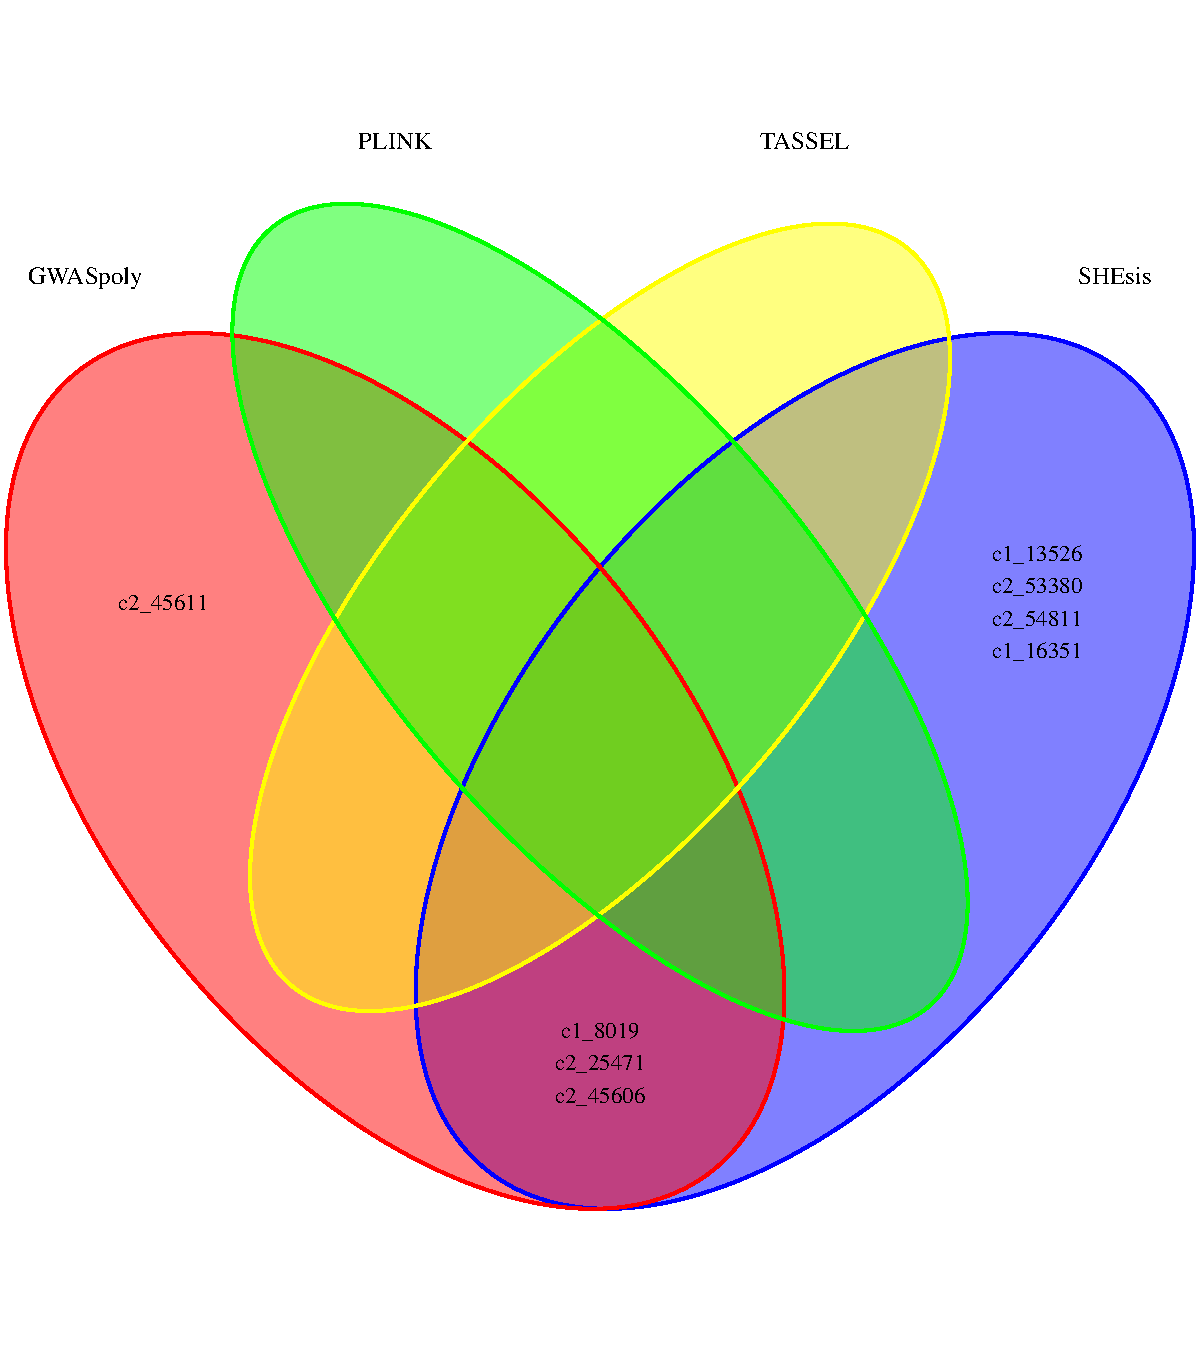
\includegraphics[bb=0bp 65bp 575bp 585bp,clip,scale=0.3]{images/out-multiGWAS-vennDiagram-significatives}
\par\end{flushleft}%
\end{minipage}

}
\par\end{centering}
\caption{\textbf{\scriptsize{}MultiGWAS views for significant SNPs.}{\scriptsize{} (a) Table with detailed information of significant SNPs found by package and sorted by decreasing score (computed as $-log_{10}(pvalue)$). The information includes: package reporting the SNP, GWAS model used by the package, chromosome, position in the genome, name or ID, score, threshold to consider the SNP as significant, and TRUE of FALSE wether the SNP is statistically significant or not (score > threshod). (b) Venn diagram with the SNPs found significant either for one package or for more than one. SNPs found by only one package are at the top of its ellipse, while SNPs found by more than one package (shared) are at the intersections of their ellipses.} {\scriptsize{}For example, the SNP c2\_45611 at the top left was found significant only by one tool: GWASpoly, but the three SNPs c1\_8019, c2\_25471, and c2\_45606, were found significative by both packages GWASpoly and SHEsis. However, the other packages, PLINK and TASSEL, did not report any significant SNP.}\label{fig:view-significatives}}
\end{figure}


\subsection{Visualization of best-ranked SNPs }

Most GWAS packages compute differently both \emph{pvalues }and significance levels, and these values may be computed either to high or to low, respectively. This results in SNPs with low \emph{pvalues }but that did not reach the significance levels defined by the packages.  Consequently, as it is important to know the significant SNPs, it is equally important to know these SNPs closer to being statistically significant, as they may represent important associations to consider for posterior analysis (e.g. false negatives).

As in the previous section, MultiGWAS tool provides a table and a Venn diagram to report these best-ranked SNPs for each GWAS package, wheter these SNPs were assesed significant or not. The number of SNPs to be reported is defined by the user in the configuration file, and these SNPs are listed in the table by tool in order of decreasing score, whereas the Venn diagram visually shows the same SNPs but emphasizing if these were best-ranked either in a single package or in several at once. Figure \ref{fig:view-best-ranked} shows the MultiGWAS best-ranked SNPs resulting from GWAS analysis on the tetraploid potato dataset.

 

\begin{figure}[H]
\begin{tabular}{cc}
\begin{minipage}[t][1\totalheight][c]{0.5\columnwidth}%
\renewcommand{\arraystretch}{1.5}
\setlength{\tabcolsep}{0.2em}
\tiny

\begin{tabular}{|c|c|c|c|c|c|c|c|}
\hline 
PKG & MDL & CHR & POS & SNP & SCR & THR & SGN\tabularnewline
\hline 
GWASpoly & Full & 10 & 48863165 & c1\_8019 & 4.7800 & 4.2500 & TRUE\tabularnewline
\hline 
GWASpoly & Full & 10 & 48808404 & c2\_25471 & 4.5700 & 4.2700 & TRUE\tabularnewline
\hline 
GWASpoly & Full & 10 & 48203431 & c2\_45611 & 4.3600 & 4.2700 & TRUE\tabularnewline
\hline 
\textcolor{blue}{GWASpoly} & \textcolor{blue}{Full} & \textcolor{blue}{10} & \textcolor{blue}{48218826} & \textcolor{blue}{c2\_45606} & \textcolor{blue}{4.6800} & \textcolor{blue}{4.5000} & \textcolor{blue}{TRUE}\tabularnewline
\hline 
.... & .... & .... & .... & .... & .... & .... & ....\tabularnewline
\hline 
PLINK & Full & 10 & 67293176 & c1\_16001 & 1.7693 & 3.2601 & FALSE\tabularnewline
\hline 
PLINK & Full & 10 & 69323144 & c2\_45611 & 1.0229 & 3.2553 & FALSE\tabularnewline
\hline 
PLINK & Full & 2 & 41814861 & c2\_16350 & 0.9598 & 3.3010 & FALSE\tabularnewline
\hline 
\textcolor{blue}{PLINK} & \textcolor{blue}{Full} & \textcolor{blue}{10} & \textcolor{blue}{69311500} & \textcolor{blue}{c2\_45606} & \textcolor{blue}{0.8489} & \textcolor{blue}{3.2923} & \textcolor{blue}{FALSE}\tabularnewline
\hline 
.... & .... & .... & .... & .... & .... & .... & ....\tabularnewline
\hline 
SHEsis & Full & 2 & 13697423 & c1\_8019 & 9.4711 & 3.3010 & TRUE\tabularnewline
\hline 
SHEsis & Full & 1 & 30837971 & c1\_13526 & 8.4501 & 3.2923 & TRUE\tabularnewline
\hline 
SHEsis & Full & 3 & 39255236 & c2\_25471 & 7.8241 & 3.2923 & TRUE\tabularnewline
\hline 
\textcolor{blue}{SHEsis} & \textcolor{blue}{Full} & \textcolor{blue}{4} & \textcolor{blue}{69311500} & \textcolor{blue}{c2\_45606} & \textcolor{blue}{5.9557} & \textcolor{blue}{3.2923} & \textcolor{blue}{TRUE}\tabularnewline
\hline 
.... & .... & .... & .... & .... & .... & .... & ....\tabularnewline
\hline 
TASSEL & Full & 10 & 47539878 & c1\_16001 & 2.2143 & 3.8943 & FALSE\tabularnewline
\hline 
TASSEL & Full & 1 & 64259758 & c2\_46195 & 2.1478 & 3.8943 & FALSE\tabularnewline
\hline 
TASSEL & Full & 1 & 63756796 & c2\_40954 & 1.9548 & 3.8943 & FALSE\tabularnewline
\hline 
\textcolor{blue}{TASSEL} & \textcolor{blue}{Full} & \textcolor{blue}{10} & \textcolor{blue}{48218826} & \textcolor{blue}{c2\_45606} & \textcolor{blue}{1.9443} & \textcolor{blue}{3.8943} & \textcolor{blue}{FALSE}\tabularnewline
\hline 
\end{tabular}%
\end{minipage} & %
\begin{minipage}[t][1\totalheight][c]{0.38\columnwidth}%
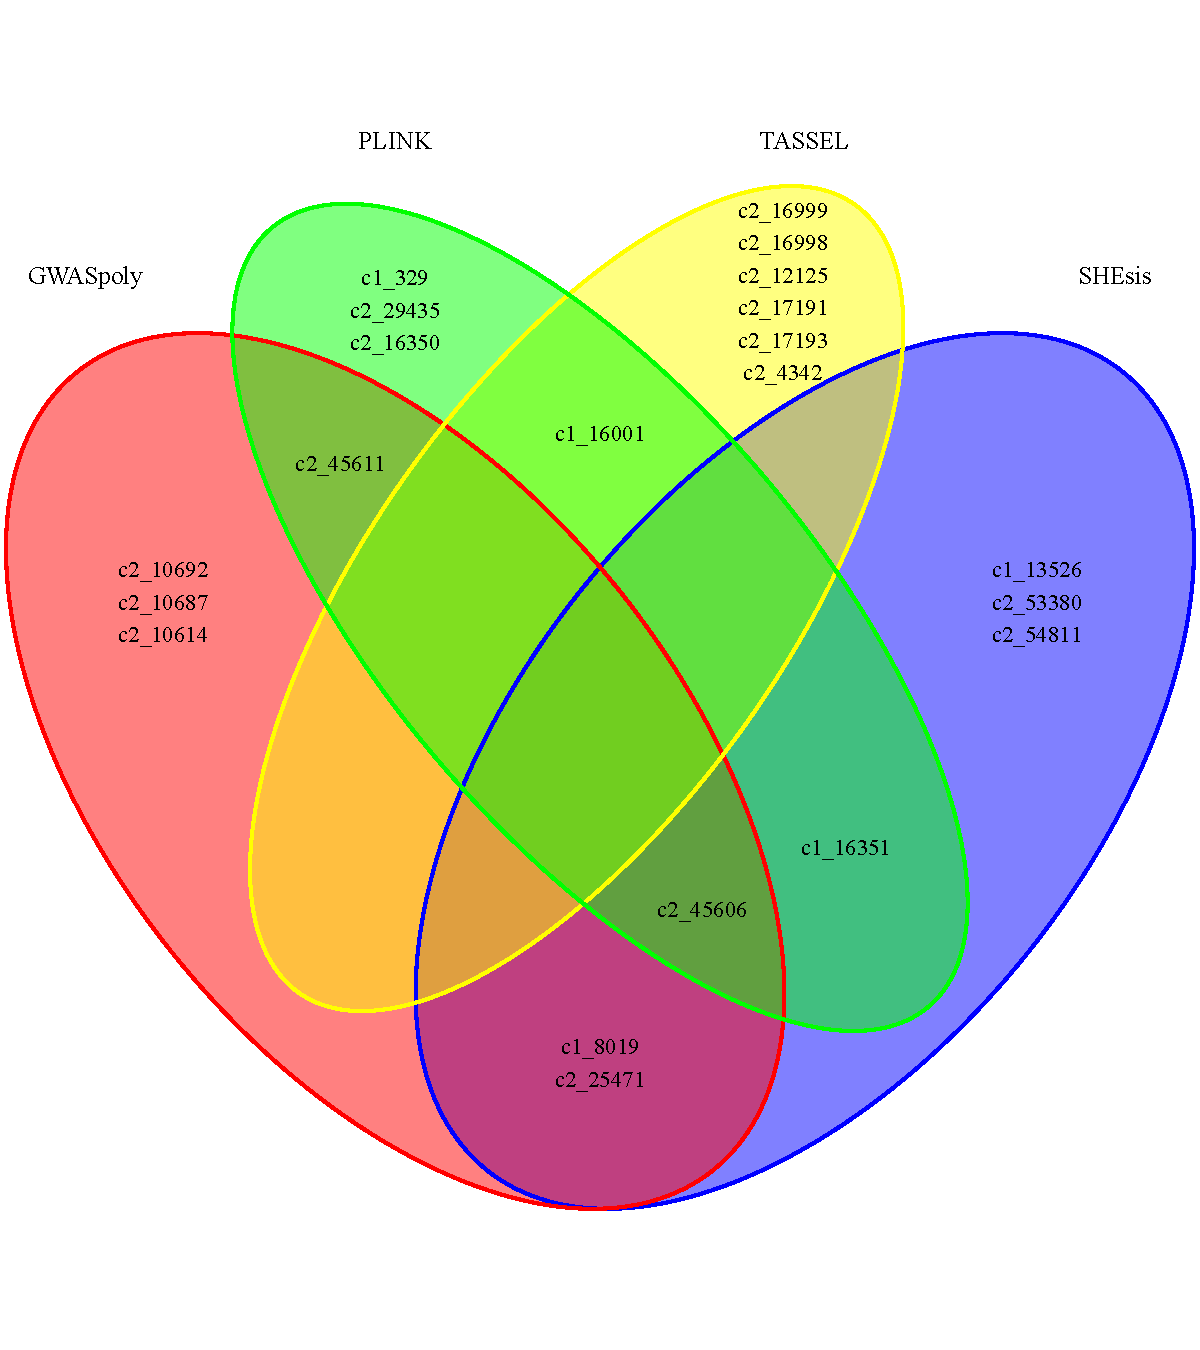
\includegraphics[bb=0bp 65bp 575bp 585bp,clip,scale=0.3]{images/out-multiGWAS-vennDiagram-best}%
\end{minipage}\tabularnewline
 & \tabularnewline
(a) & (b)\tabularnewline
\end{tabular}
\begin{centering}
\par\end{centering}
\caption{\textbf{\scriptsize{}MultiGWAS views for best-ranked SNPs.}{\scriptsize{} The views are similar to the ones described in the Figure \ref{fig:view-significatives}, but now they present a list of high-scored SNPs by package and ordered by their score. (a) Table view listing by package their first N=8 best-ranked SNPs (but only shown here four SNPs by package). (b) Venn diagram showing by package their N=8 best-ranked SNPs. One SNP was best-ranked by the four packages, c2\_45606 (central intersection of the diagram and blue highligthed row in the table). Whereas, other SNPs were best-ranked by more than one tool, c1\_8019 and 25471 (at the bottom of the diagram), were best-ranked by two packages: GWASpoly and SHEsis..\label{fig:view-best-ranked} }}
\end{figure}


\subsection{Visualization of Associations }

MultiGWAS uses classical Manhattan and Quantile\textendash Quantile plots (QQ plots) to visualize the results of GWAS analysis from each package. In both plots, SNPs are represented by dots and their $pvalues$ are transfomed to scores as $-log_{10}(pvalue)$ (see Figure \ref{fig:view-qqmanhattan}). The Manhattan plot displays the SNP association strength (y-axis) distributed in their genomic location (x-axis), so the higher the score the stronger the association. Whereas the QQ plot is used to visually compare the expected distribution of $pvalues$ (y-axis) vs. the observed distribution (x-axis), so under the null hypothesis of no association of SNPs with the phenotype, both distributions should coincide, and most SNPs should lie on a diagonal line.

\begin{figure}[H]
\subfloat[]{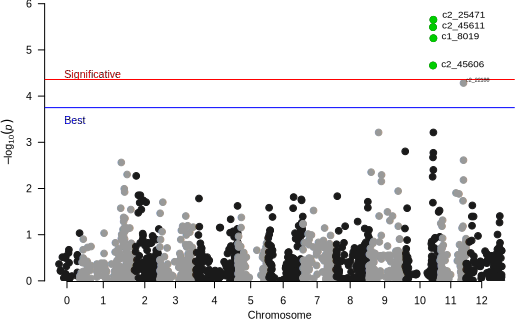
\includegraphics[scale=0.5]{images/out-multiGWAS-views-manhattan-GWASpoly}

}\subfloat[]{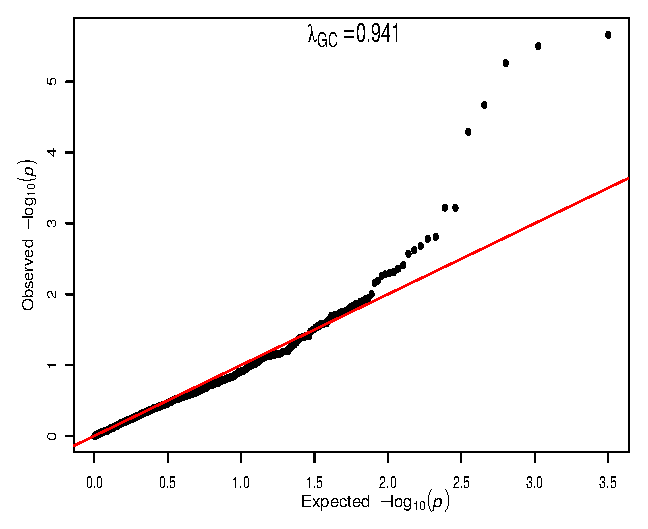
\includegraphics[scale=0.5]{images/out-multiGWAS-views-QQ-GWASpoly}

}

\caption{\textbf{\scriptsize{}MultiGWAS visualization of associations.}{\scriptsize{} MultiGWAS adds special marks to the Manhattan and QQ plots to help identify different types of SNPs: (a) In Manhattan plots, significant SNPs are above a red line, best-ranked SNPs are above a blue line, and shared SNPs (See Figure \ref{fig:view-best-ranked}) are colored in green (b) In QQ plots, a red diagonal line indicates the expectation, so potential associations can be observed when the number of SNPs deviating from the diagonal is small, as in the case of monogenic traits, or when this number is somewhat higher, as in the case of truly polygenic traits. However, deviations for a high number of SNPs could reflect inflated $pvalues$ owing to population structure or cryptic relatedness. \label{fig:view-qqmanhattan}}}

\end{figure}

\bibliographystyle{plain}
\bibliography{multiGWAS}

\begin{description}
\item [{Threshold:}]~
\begin{itemize}
\item \textbf{Rosyara2016}: 
\item \textbf{Gumpinger2018}: 
\end{itemize}
\item [{Manhattan~plots:}]~
\begin{itemize}
\item Ferrao2018: 
\item \textbf{Powel2016:} 
\item \textbf{Gumpinger2018}: 
\item Tan2016: 
\end{itemize}
\item [{QQ-plots:}]~
\begin{itemize}
\item This figure is called a Q-Q plot and can be very useful in evaluating GWAS data for systematic bias.
\item Two types of plot are used to visualize the results of genome-wide association studies (GWAS).
\item \textbf{Pearson2008: }
\item \textbf{Powel2016:} 
\item \textbf{Gumpinger2018: }
\item \textbf{Rosyara2016}: 
\item Childs2012: 
\item Tan2016: 
\end{itemize}
\item [{False\_negatives:}]~
\begin{itemize}
\item \textbf{Gumpinger2018:} 
\end{itemize}
\item [{Logarithm\_scale:}]~
\begin{itemize}
\item \textbf{Powel2016: }
\end{itemize}
\item [{GWAS\_statistical\_models:}]~
\begin{itemize}
\item Anonymous: 
\end{itemize}
\item [{Inflation\_factor:}]~
\begin{itemize}
\item \textbf{Gumpinger2018:} 
\end{itemize}
\item [{Multiple\_hypothesis\_testing:}]~
\begin{itemize}
\item Childs2012: 
\end{itemize}
\end{description}

\end{document}
